% \subsection{Objetivos específico}
\begin{frame}[allowframebreaks]
	\frametitle{Objetivo específico}
	\begin{enumerate}
		\item Realizar un estudio del estado de la cuestión sobre arquitecturas tolerantes a fallas para sistemas críticos.
		\item Investigar y analizar arquitecturas tolerantes a fallas que aseguren la confiabilidad del sistema y que sean aplicables en la industria satelital.
		\item Investigar y analizar protocolos de comunicación, para las capas superiores del modelo de OSI (modelo de interconexión de sistemas abiertos - ISO/IEC 7498-1), orientados a la tolerancia a fallas y confiabilidad de los sistemas. 
		\item Investigar una metodología para lograr una medición de la tolerancia a fallas en arquitecturas de aviónica.
		\item Desarrollar un estudio comparativo de arquitecturas tolerantes a fallas con el fin de obtener ventajas y desventajas de cada una de ellas.
		\item Diseñar modelos alternativos de arquitecturas tolerantes a fallas, que tengan un grado de confiabilidad tal, que permita la aplicación de componentes COTS.
		\item Evaluar la confiabilidad de los modelos de arquitecturas.
		\item Proponer el diseño de una nueva arquitectura tolerante a fallas, con un grado de confiabilidad suficiente para la aplicación de componentes COTS en avionicas de vehículos satelitales.
		\item Simular la arquitectura planteada para medir su grado de tolerancia a fallas y performance.
	\end{enumerate}
\end{frame}

\begin{frame}[noframenumbering, c]
	\LARGE
	\centering
	\textbf{Backup Slides}
\end{frame}

\begin{frame}
	\frametitle{Fallas != Error != Avería}
	\begin{itemize}
		\item \textbf{Avería:} ocurre cuando el servicio prestado por el sistema no coincide con las especificaciones del mismo.  Existe una consecuencia negativa en el sistema completo. (Failure)
		\item \textbf{Error:} es una parte del estado del sistema que es susceptible de provocar un avería en el sistema. Es una etapa intermedia entre falla y avería. (Error)
		\item \textbf{Falla:} también llamado “bug”. Es la hipótesis de un error. (Fault)
	\end{itemize}
\end{frame}

\begin{frame}
	\frametitle{Fallas de modo común vs fallas de causa común}
	\begin{itemize}
		\item \textbf{Fallas de modo común (CMF):}  es una falla que ocurre simultáneamente en dos o más componentes redundantes. CMF son causados por fenómenos que crean dependencias entre unidades redundadas.
		\item \textbf{Fallas de causa común (CCF):} se define como cualquier instancia donde múltiples elementos fallan debido a una causa común
	\end{itemize}
\end{frame}

\begin{frame}
	\frametitle{Fallas en el Software}
	Algunas de las fallas introducidas en el software:
	\begin{itemize}
		\item Especificaciones incorrecta de requerimientos
		\item Diseño incorrecto
		\item Errores de programación
	\end{itemize}
\end{frame}

\begin{frame}
	\frametitle{Fiabilidad de sistemas}
	La fiabilidad de un sistema es la capacidad del mismo de entregar a los usuarios un nivel deseado de servicio. 
	\vfill
	Es una medida de calidad que abarca los conceptos: confiabilidad, disponibilidad, y seguridad.
	\vfill
	Es un propiedad global que permite justificar la confianza de los servicios de un sistema 
	
\end{frame}

\begin{frame}
	\frametitle{Medios de fiabilidad}
	\begin{itemize}
		\item \textbf{Evitación de fallas:} técnicas de mejoramiento de la fiabilidad utilizadas durante el desarrollo de SW para reducir el número de fallas.  
		\item \textbf{Tolerancia a fallas:} se utiliza como una capa más de protección. FT es la capacidad del sistema a ejecutarse apropiadamente a pesar de la presencia de fallas. FT ocurre en tiempo de ejecución.
		\item \textbf{Eliminación de Fallas:} técnicas utilizadas para mejorar la fiabilidad empleadas durante el proceso de validación y verificación del sistema SW. Se eliminan la fallas que se detectan.
		\item \textbf{Predicción de Fallas:} se aplica mediante la realización de una evaluación del comportamiento del sistema con respecto a la ocurrencia, o la activación de una falla.
	\end{itemize}
\end{frame}

\begin{frame}
	\frametitle{Failure rate}
	Es el número esperado de fallas por unidad de tiempo. Generalmente, se encuentra a nivel de componente.
	\LARGE
	$$
	\lambda =  \sum_{i=1}^{n} \lambda_n
	$$	
\end{frame}

\begin{frame}
	\frametitle{Failure rate}
	\begin{columns}[T]
		\begin{column}{.5\textwidth}
			\centering
			Failure rate de HW vs tiempo
			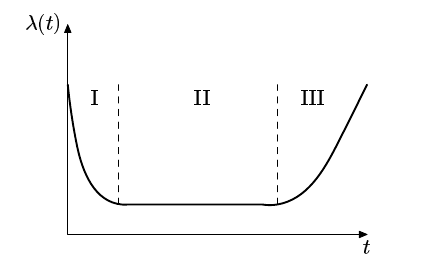
\includegraphics[scale=0.4]{images/bathtub_curve.png}
		\end{column}
		\begin{column}{.5\textwidth}
			\centering
			Failure rate de SW vs tiempo
			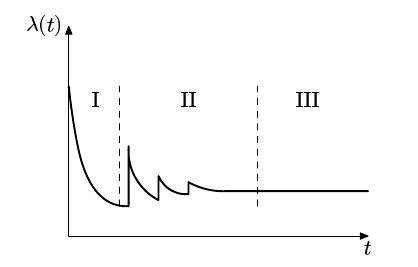
\includegraphics[scale=0.4]{images/Failure_rate_software.png}
		\end{column}
	\end{columns}
\end{frame}

\begin{frame}
	\frametitle{Failure rate}
	\textbf{Tiempo medio hasta la falla (MTTF):}
	$$ MTTF = \int_{0}^{\infty}{R(t) dt} $$
	\textbf{Tiempo medio de reparación (MTTR):}
	$$ MTTR = 1/\mu $$
\end{frame}

\begin{frame}
	\frametitle{Redundancia en el software}
	\begin{itemize}
		\item Técnicas single version
		\item Técnicas multi-version
		\item Técnicas de detección de fallas
		\item Técnicas de recuperación de fallas
	\end{itemize}
\end{frame}